\graphicspath{{Figs/montecarlo/}}

%
% To start the document, use
%  \chapter{...}
% For lover level, sections use
%  \section{...}
%  \subsection{...}
%
\chapter{Reversed Monte Carlo Scattering: ARTS-MC}
 \label{sec:montecarlo}


%
% Document history, format:
%  \starthistory
 %    date1 & text .... \\
%    date2 & text .... \\
%    ....
%  \stophistory
%
\starthistory
  120410 & Moved from user guide to theory document.\\
  300504 & Created and written by Cory Davis.\\
\stophistory


%
% Symbol table, format:
%  \startsymbols
%    ... & \verb|...| & text ... \\
%    ... & \verb|...| & text ... \\
%    ....
%  \stopsymbols
%
%

%
% Introduction
%




\section{Introduction}
 \label{sec:montecarlo:intro}

PDFS are chosen to be well suited to calculating the 1st component of
the Stokes vector.

%%%%%%%%%%%%%%%%%%%%%%%%%%%%%%%%%%%%%%%%%%%%%%%%%%%%%%%%%% 
\section{Model}
 \label{sec:montecarlo:model}
The radiative transfer model solves the vector
radiative transfer equation (VRTE):
\begin{eqnarray}
\frac{d\mathbf{I(n)}}{ds}=-\mathbf{K(n)I(n)} +
\mathbf{K_a(n)}I_b(T) +\nonumber\\
\int_{4\pi}\mathbf{Z(n,n')I(n')}d\mathbf{n'}
\label{vrte}
\end{eqnarray}
where $\mathbf{I}$ is the 4 element column vector of radiances
$\mathbf{I}=\left[I,Q,U,V\right]^T$ with units
(Wm$^{-2}\mu$m$^{-1}$sr$^{-1}$). This will be referred to as the
Stokes vector, although normally the Stokes vector is expressed in
units of intensity.  $s$ is distance along direction $\mathbf{n}$ and
$I_b$ is the Planck radiance. $\mathbf{K(n)}$, $\mathbf{K_a(n)}$,
and $\mathbf{Z(n,n')}$ are the bulk extinction matrix, absorption
coefficient vector and phase matrix of the medium respectively.  For
 brevity these have been expressed as bulk optical
properties, where individual single scattering properties have been
multiplied by particle number density and averaged over all
orientations and particle types. The argument $\mathbf{n}$ has been
retained to signify that in general these properties depend on the
direction of propagation. 

To apply Monte Carlo integration to the problem, the VRTE needs to be expressed in integral form. (e.g. \cite{hochstadt:64})
\begin{eqnarray}
\lefteqn{\mathbf{I(n,s_0)}=\mathbf{O(u_0,s_0)I(n,u_0)}+}\nonumber\\
& \int_{u_0}^{s_0}\mathbf{O(s',s_0)}\left(\mathbf{K_a(n)}I_b(T) +\int_{4\pi}\mathbf{Z(n,n')}\mathbf{I(n')}d\mathbf{n'}\right)ds'\nonumber
\end{eqnarray}
\begin{equation}
\label{intVRTE}
\end{equation}
, where $\mathbf{O(s',s)}$ is the evolution operator defined by
\cite{landi:85}. $\mathbf{u_0}$ is the point where the line of sight intersects
the far boundary of the scattering domain, and $\mathbf{s_0}$ is the
exit point where the outgoing Stokes vector is calculated.

\subsection{Integration over the antenna response function}

If we consider a scalar antenna response function,
$\psi=\psi(\theta,\phi)=\psi(\mathbf{n})$, where $\psi(\mathbf{n})$ is
normalised such that $\int_{4\pi}\psi(\mathbf{n})dn=1$, then the
observed Stokes vector $\mathbf{I_{ant.}(n,s_0)}$ will be

\begin{equation}
\mathbf{I_{ant.}(n,s_0)}=\int_{4\pi}\psi(\mathbf{n'})\mathbf{I(n',s_0)}d\mathbf{n'}
\label{antInt}
\end{equation}

If we apply Monte Carlo integration with importance samping to
Eq. \ref{antInt} and sample $\mathbf{n'}$ according to a probability
density function (PDF) equal to $\psi(\mathbf{n'})$, an unbiased
estimate of Eq. \ref{antInt} is given by (e.g. \cite{press:92})

\begin{eqnarray}
\mathbf{I_{ant.}(n,s_0)}&=&\int_{4\pi}\mathbf{I(n',s_0)}\psi(\mathbf{n'})d\mathbf{n'}\\
&=&\langle \mathbf{I(n',s_0)} \rangle_\psi
\label{antIntMC}
\end{eqnarray}
, with an estimated error for each Stokes index, $j$,  of
\begin{equation}
\delta I_j=\sqrt{\frac{\langle I_j^2\rangle-\langle I_j\rangle^2}{N}}.
\label{error}
\end{equation}
\subsection{The path integral}

We now require a Monte Carlo estimate of the integrand in
Eq. \ref{antIntMC}, which is given by Eq. \ref{intVRTE}.  First, we
re-express \ref{intVRTE} as a single integral, for simplicity dropping
the prime on $\mathbf{n'}$,

\begin{equation}
\mathbf{I(n,s_0)}=\int^{s_0}_\infty\left\{\begin{array}{rl}
\mathbf{O(s',s_0)}\left(\mathbf{K_a(n)}I_b(T)
+\int_{4\pi}\mathbf{Z(n,n')}\mathbf{I(n')}d\mathbf{n'}\right) & s'< s'_{boundary} \\
\frac{\mathbf{O(u_0,s_0)I(n,u_0)}g}{\int^\infty_{u_0}gds} & s'\ge s'_{boundary}
\end{array}ds'\right.
\label{inorouteq}
\end{equation}
, where $g$ is the PDF we will eventually use to sample pathlength,
$\Delta s$. $s'_{boundary}$ represents the pathlength corresponding to
the boundary of the domain opposite the line of sight.
The integrand Eq. \ref{inorouteq} is a piecewise function of the
path distance, where path distances corresponding to positions outside
the modelled domain give a boundary radiance attenuated by evolution
operator over the length of the path within the model domain, and path
distances corresponding to points within the modelled atmosphere give
a sum of emission and scattering attenuated by the evolution operator
over the distance between the point and the atmosphere exit. 
The reader
could easily verify that evaluating Eq. \ref{inorouteq} is equivalent
Eq. \ref{intVRTE}. 

The aim in importance sampling is to choose probability density functions
(PDFs) for the independent variables that are
as close as possible to being proportional to the integrand
\cite{liu:01}. This concentrates computational effort on regions where
the integrand is most significant and also reduces the variance in the contributions of each photon, thus reducing
the number of photons and hence CPU time required to give a
prescribed accuracy.  Eq. \ref{intVRTE} suggests that the PDF for
sampling path length, where path length is the distance traced backwards
from the sensor, $\Delta s=\left|\mathbf{s}-\mathbf{s'}\right|$, should be proportional in some way to the evolution
operator $\mathbf{O(s',s)}$. 

In general there is no closed form expression for $\mathbf{O(s',s)}$.
However, in cases where the extinction matrix is constant along a
propagation path
\begin{equation}
\mathbf{O(s',s)}=\exp\left(-\mathbf{K}\Delta s\right)
\label{OconstK}
\end{equation}
In ARTS a propagation path consists of a set of coordinates
indicating where the path intersects with grid surfaces.  If the
extinction matrix in the path segment between two such points is
considered constant, $\mathbf{K}=(\mathbf{K_j}+\mathbf{K_{j+1}})/2$,
the evolution operator between two arbitrary points $\mathbf{s_0}$ and
$\mathbf{s}_N$ is
\begin{eqnarray}
\mathbf{O}(\mathbf{s}_0,\mathbf{s}_N) =
\mathbf{O}(\mathbf{s}_{N-1},\mathbf{s}_N)
\mathbf{O}(\mathbf{s}_{N-2},\mathbf{s}_{N-1}) \dots \nonumber\\
\mathbf{O}(\mathbf{s}_1,\mathbf{s}_2)\mathbf{O}(\mathbf{s}_0,\mathbf{s}_1),
\label{Ogeneral}
\end{eqnarray}
, where $\mathbf{O(s_i,s_{i+1})}$ is given by Eq. \ref{OconstK}.

Since PDFs are scalar functions, and that we consider the first element of the
Stokes vector most important, we choose the pathlength PDF to be proportional to the
(1,1) element of $\mathbf{O(s',s)}$,

\begin{equation}
g(\Delta s)=\tilde{k}\tilde{O_{11}}(\Delta s)
\label{gDeltas}
\end{equation}
This is sampled by taking a random number and solving 
\begin{equation}
\tilde{O_{11}}(\Delta s)=r.
\label{solvefor0}
\end{equation}
for $\Delta s$.  Here, 
\begin{equation}
\tilde{k}=\frac{1}{\left(\Delta s_B-\Delta s_A\right)}
\ln\left(\frac{O_{11}^A}{O_{11}^B}\right)
\end{equation}
, which, for cases where the extinction matrix is diagonal, is equal to $K_{11}=(K_{11}^A+K_{11}^B)/2$.

With pathlength sampled according to Eq. \ref{solvefor0}, the Monte
Carlo estimate for Eq. \ref{inorouteq} becomes
\begin{eqnarray}
\mathbf{I(n,s_0)}&=&\int^{s_0}_\infty\left\{\begin{array}{rl}
\frac{\mathbf{O(s',s_0)}}{g(\Delta s)}\left(\mathbf{K_a(n)}I_b(T)
+\int_{4\pi}\mathbf{Z(n,n')}\mathbf{I(n')}d\mathbf{n'}\right) & s'< s'_{boundary} \\
\frac{\mathbf{O(u_0,s_0)I(n,u_0)}}{1-\tilde{O_{11}}(\Delta s)} & s'\ge s'_{boundary}
\end{array}g(\Delta s)ds'\right.\nonumber\\
&\approx&\left\langle\left\{\begin{array}{rl}
\frac{\mathbf{O(s',s_0)}}{g(\Delta s)}\left(\mathbf{K_a(n)}I_b(T)
+\int_{4\pi}\mathbf{Z(n,n')}\mathbf{I(n')}d\mathbf{n'}\right) & s'< s'_{boundary} \\
\frac{\mathbf{O(u_0,s_0)I(n,u_0)}}{1-\tilde{O_{11}}(\Delta s)} & s'\ge s'_{boundary}
\end{array}\right.\right\rangle_{g(\Delta s)}
\label{pathlengthint}
\end{eqnarray} 

So if the sampled pathlength corresponds to a point outside the
atmosphere, or below the earth' surface, the Monte Carlo estimator (is this
the right word) is given by
$\frac{\mathbf{O(u_0,s_0)I(n,u_0)}}{1-\tilde{O_{11}}(\Delta s)}$. In the
top of atmopshere cases, this can be immediately calculated:
$\mathbf{O(u_0,s_0)}$ from Eq. \ref{Ogeneral}, and $\mathbf{I(n,u_0)}$ from
  the background radiation from space.  As shown in Figure
  \ref{fig:montecarlo:flowchart}, in this event, we have our Monte
  Carlo contribution and we can begin the calculation for the next
  one.  If however the reversed traced path passes the surface, the
  calculation of $\mathbf{I(n,u_0)}$ requires more steps.

\subsection{Emission and scattering}

If the sampled pathlength corresponds to a point within the
atmosphere then the emission and scattering terms in the top term in
Eq. \ref{pathlengthint}, must be calculated.  We also treat this as
Monte Carlo integration:
\begin{eqnarray}
\mathbf{K_a(n)}I_b(T)
+\int_{4\pi}\mathbf{Z(n,n')}\mathbf{I(n')}d\mathbf{n'}&=&\int_0^1\left\{\begin{array}{rl}\frac{1}{\tilde{\omega}}\int_{4\pi}\mathbf{Z(n,n')}\mathbf{I(n')}d\mathbf{n'}
& r \le \tilde{\omega}\\
\frac{\mathbf{K_a(n)}I_b(T)}{1-\tilde{\omega}}& r >
\tilde{\omega}\end{array}dr\right.\nonumber\\
&\approx&\left\langle\left\{\begin{array}{rl}\frac{1}{\tilde{\omega}}\int_{4\pi}\mathbf{Z(n,n')}\mathbf{I(n')}d\mathbf{n'}
& r \le \tilde{\omega}\\
\frac{\mathbf{K_a(n)}I_b(T)}{1-\tilde{\omega}}& r >
\tilde{\omega}\end{array}\right.\right\rangle_r
\label{emiss-or-scatter}
\end{eqnarray}.
Here we are using a uniform random deviate $r$, and an
albedo-like quantity,
\begin{equation}
\tilde{\omega}=1-\frac{K_{a1}(\mathbf{n_{0},s_{1}})}{K_{11}(\mathbf{n_{0},s_{1}})}
\end{equation}
, to choose between emission and scattering contributions.
Note: we can't use the actual single-scattering albedo as this depends
on the polarization state of the incident radiation.  If
$r>\tilde{\omega}$, then the event is considered to be emission.  In
this case we have all the information required to calculate the Monte
Carlo estimator,
\begin{equation}
\mathbf{I^i(n,s_0)}=\frac{\mathbf{Q_k O(s_{k+1},s_k)}
  \mathbf{K_a(n_k,s_{k+1})} I_b(T,\mathbf{s_{k+1}})}
  {g\left(\Delta s\right)\left(1-\tilde{\omega}\right)}
\label{Iemission}
\end{equation}
, where $\mathbf{O(s_{k+1},s_k)}$ is the evolutaion operator
pertaining to the preceding pathlength sample, and $g\left(\Delta
s\right)$, the corresponding importance sampling weight, as indicated
in Eq. \ref{pathlengthint}.  The matrix $\mathbf{Q_k}$, whose
calculation will be described below, holds the
multiplicative effect of previous evolution operators, phase matrices,
surface reflection matrices, and importance sampling weighting
factors, acting on the reversed traced multiply scattered propagation
path. 

\subsection {The scattering integral}

If, in Eq. \ref{emiss-or-scatter} our sampled $r\le\tilde{\omega}$
, we have a scattering event.  In this case we need to evaluate the scattering
integral $\int_{4\pi}\mathbf{Z(n,n')}\mathbf{I(n')}d\mathbf{n'}$.
Again we apply Monte Carlo integration with importance sampling to
this integral.
\begin{eqnarray}
\int_{4\pi}\mathbf{Z(n,n')}\mathbf{I(n')}d\mathbf{n'}&=&\int_0^{2\pi}\int_0^\pi\frac{\mathbf{Z(n,n')}\mathbf{I(n')}}{g(\theta_{inc},\phi_{inc})}g(\theta_{inc},\phi_{inc})\sin{\theta_{inc}}d\theta_{inc}d\phi_{inc}\\
&\approx&\left\langle\frac{\sin{\theta_{inc}}\mathbf{Z(n,n')}\mathbf{I(n')}}{g(\theta_{inc},\phi_{inc})}\right\rangle_{g(\theta_{inc},\phi_{inc})}
\label{scattering_int}
\end{eqnarray}
Given the desire to use a PDF proportional to the integrand, we
choose to sample incoming directions,
$\mathbf{n'}=(\theta_{inc},\phi_{inc})$ from a PDF proportional
to $\sin{\theta_{inc}}\mathbf{Z}(\theta_{scat},\phi_{scat},\theta_{inc},\phi_{inc})$.
At the scattering point sample a new incident direction
  $(\theta_{inc},\phi_{inc})$ according to 
\begin{equation}
g(\theta_{inc},\phi_{inc})=\frac{Z_{11}(\theta_{scat},\phi_{scat},
\theta_{inc},\phi_{inc})\sin(\theta_{inc})}{K_{11}(\theta_{scat},\phi_{scat})
  - K_{a1}(\theta_{scat},\phi_{scat})}
\label{gdir}
\end{equation}
, which is
sampled by the rejection method as described in \cite{liu:01}.  This sampling of the new incoming direction for the evaluation of Eq. \ref{scattering_int} leads to the calculation of the incoming stokes vector $\mathbf{I(n',s)}$ at the point of scattering $\mathbf{s}$ in the new incident direction $\mathbf{n'}$. We thus return to pathlength sampling and evaluation of Eq. \ref{pathlengthint}.  

\subsection{Applying the Mueller matrices}

The influence of the phase matrix and the preceding evolution operator, along with the importance samping weights, are stored by calculating the matrix
\begin{equation}
\mathbf{Q_k}=\mathbf{Q_{k-1}q_k}
\label{Q}
\end{equation}
, where
\begin{equation}
\mathbf{q_k}=\frac{\sin(\theta_{inc})_k
  \mathbf{O(s_k,s_{k-1})}\mathbf{Z(n_{k-1},n_k)}}
  {g\left(\Delta s\right)g(\theta_{inc},\phi_{inc}) \tilde{\omega}} ,
\label{q}
\end{equation}
and $\mathbf{Q_0}={1}$. The index $k$ represents the
scattering order.  The $\mathbf{Q_k}$ is updated through subsequent scattering events and finally applied to an emission contribution (Eq. \ref{Iemission}) if an emission event is sampled in Eq. \ref{emiss-or-scatter}.  

\subsection {Boundary contributions}

Similarly, if the $k$\textsuperscript{th} pathlength sampled in Eq. \ref{pathlengthint} is beyond the top of the atmosphere or below the earth surface, $\mathbf{Q_k}$ is applied in 
\begin{equation}
\mathbf{I^i(n,s_0)}=\frac{\mathbf{Q_k}\mathbf{O(u_k,s_k)I(n_k,u_k)}}{O_{11}(\mathbf{u_{k},s_k})}
\label{Ikmax2_1}
\end{equation}
, where 
$\mathbf{I(n_k,u_k)}$ is the incoming radiance at boundary point $\mathbf{u}_{k}$.  For the top of atmosphere case, $\mathbf{I(n_k,u_k)}=I_{space}$.  In ARTS it is possible to set $I_{space}$ to any value, but in most cases this is set to the cosmic background radiance associated with a Planck temperature of 2.735K. 

For the surface case, if we choose to treat the surface as a blackbody, i.e. there is no reflection, in Eq. \ref{Ikmax2_1} we set $\mathbf{I(n_k,u_k)}=I_{surf}$, where $I_{surf}$ is the Planck radiance associated with the surface temperature, $I_{surf}=I_b{T_{surf}}$. 

\subsection{Surface reflection} 

Currently ARTS-MC can only consider specular reflection.  \emph{It would be a straightforward development to handle more complicated reflectins.  In the same way that the phase matrix is sampled to choose new incoming directions for scattering events, we could sample the Bidirectional reflection distribution (BDRF) for surface reflection events.} In analogy with scattering and emission in Eq. \ref{emiss-or-scatter}, $\mathbf{I_{surf}}$ is given by the sum of reflected and emitted radiation:

\begin{eqnarray}
\mathbf{I_{surf}(n_k,u_k)}&=&\mathbf{B(n_k,u_k)}+\mathbf{R(n_k,n_{k+1},u_k)I(n_{k+1},u_k)}\nonumber\\
&=&\int^1_0\left\{\begin{array}{rl}\frac{1}{R_{11}}\mathbf{R(n_k,n_{k+1},u_k)I(n_{k+1},u_k)} & r \le R_{11}\\
\frac{\mathbf{B(n_k,u_k)}}{1-R_{11}}& r > R_{11}\end{array}dr\right.\nonumber\\
&\approx&
\left\langle\left\{\begin{array}{rl}\frac{1}{R_{11}}\mathbf{R(n_k,n_{k+1},u_k)I(n_{k+1},u_k)} & r \le R_{11}\\
\frac{\mathbf{B(n_k,u_k)}}{1-R_{11}}& r > R_{11}\end{array}\right.\right\rangle_r
\label{I_surf}
\end{eqnarray}

The reflection matrix $\mathbf{R(n_k,n_{k+1},u_k)}$ and related surface emission, $\mathbf{B(n_k,u_k)}$ are calculated in one of several ways, as described in section {\bf[FIXME: that stuff should be in this document but it isn't yet]}.  As in Eq. \ref{emiss_or_scatter}, we use a uniform random deviate $r$; if
$r>R_{11}$, where $R_{11}$ is the (1,1) element of $\mathbf{R(n_k,n_{k+1},u_k)}$, then the event is considered to be surface emission.  In
this case we have all the information required to calculate the Monte
Carlo estimator in Eq.\ref{Ikmax2_1} becomes, 
\begin{equation}
\mathbf{I^i(n,s_0)}=\frac{\mathbf{Q_k}\mathbf{O(u_k,s_k)B(n_k,u_k)}}{O_{11}(\mathbf{u_{k},s_k})(1-R_{11})}.
\label{Ikmax2_2}
\end{equation}

NEXT THE REFLECTION CASE AND FIX THE FLOWCHART

\begin{figure}
\begin{center}
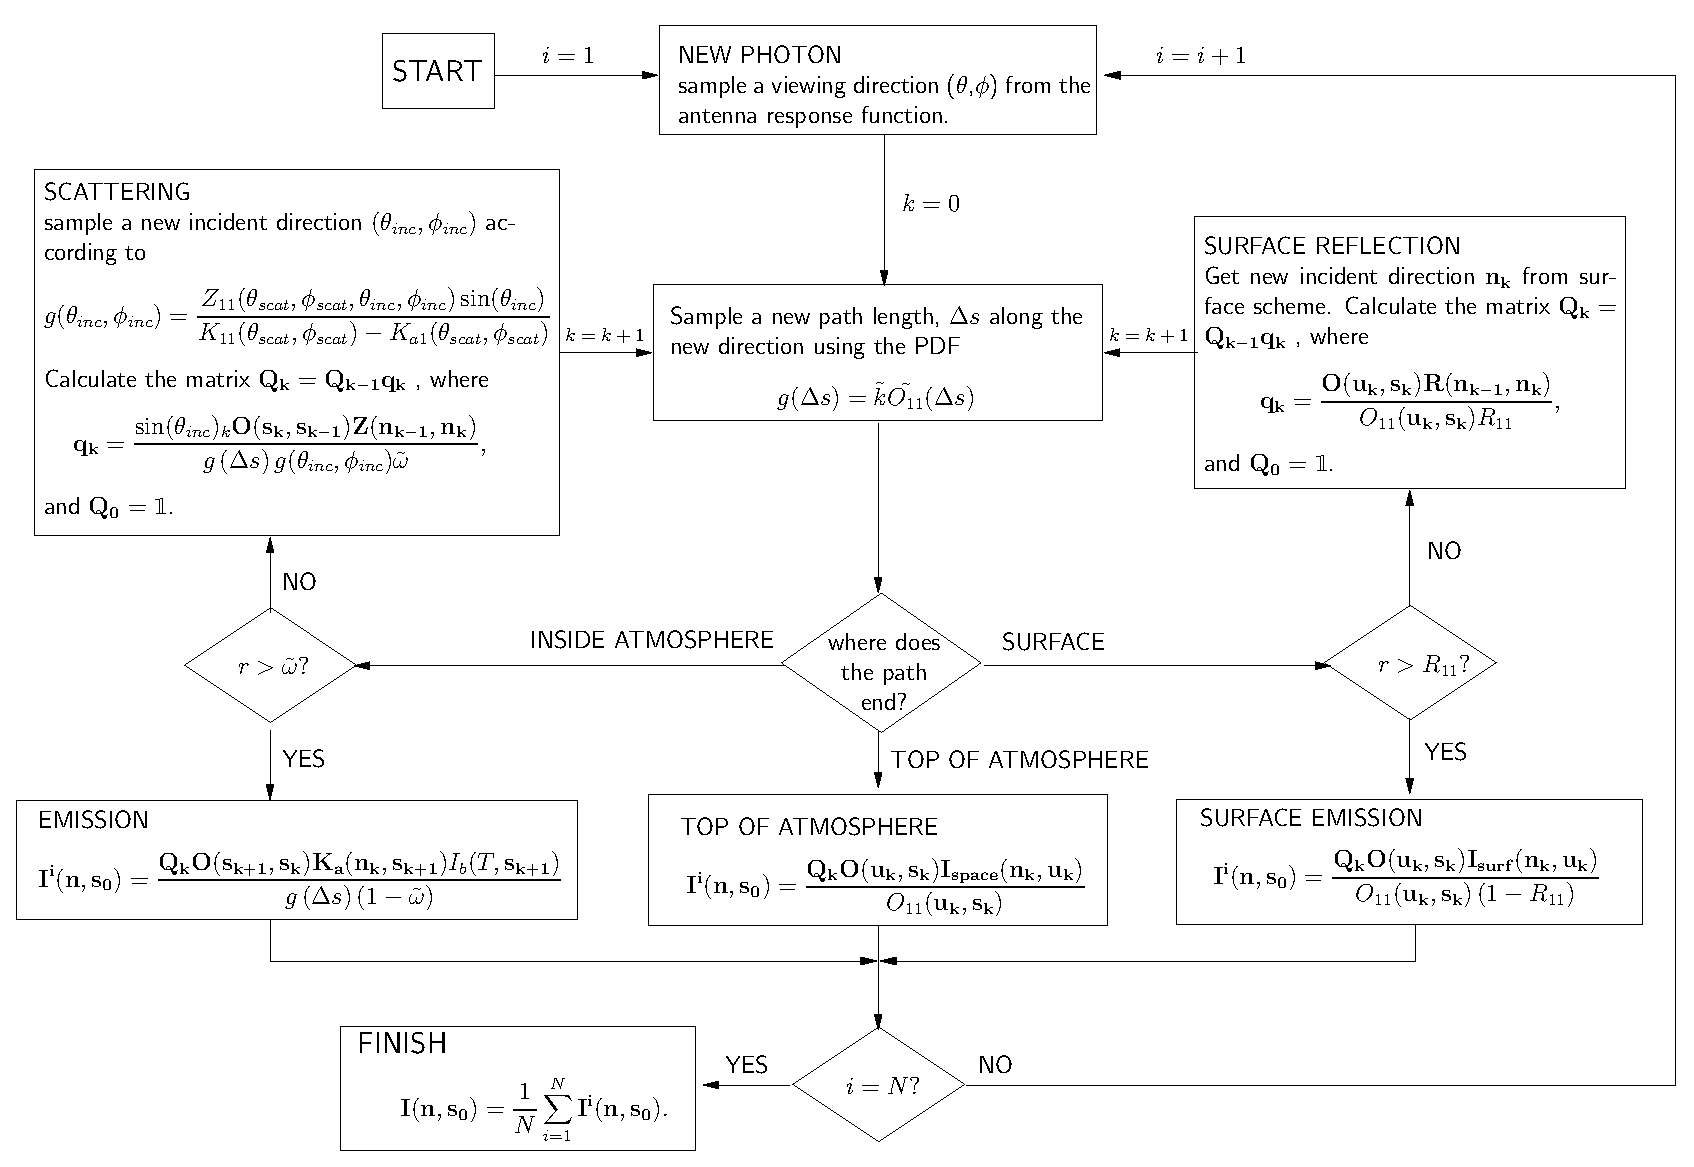
\includegraphics[width=\vsize,angle=90]{flowchart2}
\caption{Flowchart illustrating MCGeneral algorithm}
\end{center}
\label{fig:montecarlo:flowchart}
\end{figure}

 
%%% Local Variables: 
%%% mode: latex 
%%% TeX-master: "uguide" 
%%% End:

